% Generated by experiments/icpc/make_result_figs.py from committed results. Do not edit by hand.
\documentclass[border=2pt]{standalone}
\usepackage[T1]{fontenc}\usepackage{newtxtext,newtxmath}\usepackage[varqu,scaled=0.95]{zi4}
\usepackage{pgfplots}\pgfplotsset{compat=1.18}
\definecolor{cblue}{HTML}{0072B2}\definecolor{cver}{HTML}{D55E00}\definecolor{cora}{HTML}{E69F00}
\definecolor{cgreen}{HTML}{009E73}\definecolor{cgrey}{HTML}{999999}\definecolor{csky}{HTML}{56B4E9}\definecolor{cpurple}{HTML}{7E57C2}
\pgfplotsset{every axis/.append style={font=\footnotesize, tick label style={font=\scriptsize},
  label style={font=\footnotesize}, legend style={font=\scriptsize, draw=none, fill=none},
  axis lines*=left, ymajorgrids, grid style={black!8}}}
\begin{document}
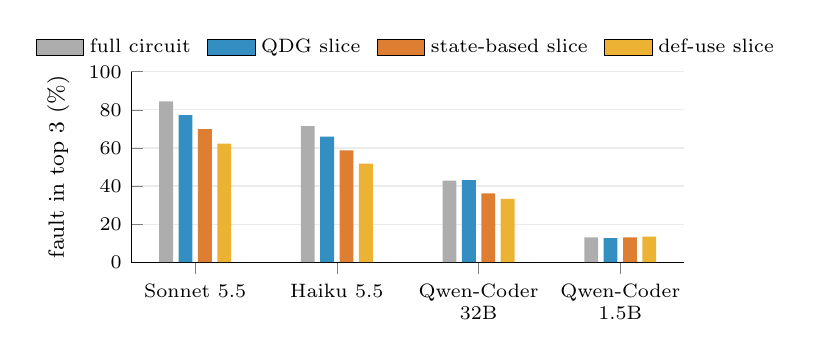
\begin{tikzpicture}\begin{axis}[ybar, bar width=5pt, width=8.6cm, height=4.0cm, ymin=0, ymax=100,
 ylabel={fault in top 3 (\%)}, symbolic x coords={Sonnet 5.5,Haiku 5.5,Qwen-Coder 32B,Qwen-Coder 1.5B}, xtick=data, enlarge x limits=0.15,
 xticklabels={{Sonnet 5.5},{Haiku 5.5},{Qwen-Coder\\32B},{Qwen-Coder\\1.5B}}, xticklabel style={align=center},
 legend style={at={(0.5,1.02)}, anchor=south, legend columns=4, /tikz/every even column/.append style={column sep=4pt}}, area legend]
\addplot[fill=cgrey!80, draw=none] coordinates {(Sonnet 5.5,84.4) (Haiku 5.5,71.4) (Qwen-Coder 32B,42.8) (Qwen-Coder 1.5B,13.0)};
\addplot[fill=cblue!80, draw=none] coordinates {(Sonnet 5.5,77.2) (Haiku 5.5,65.9) (Qwen-Coder 32B,43.1) (Qwen-Coder 1.5B,12.7)};
\addplot[fill=cver!80, draw=none] coordinates {(Sonnet 5.5,69.9) (Haiku 5.5,58.7) (Qwen-Coder 32B,36.2) (Qwen-Coder 1.5B,13.0)};
\addplot[fill=cora!80, draw=none] coordinates {(Sonnet 5.5,62.3) (Haiku 5.5,51.8) (Qwen-Coder 32B,33.3) (Qwen-Coder 1.5B,13.4)};
\legend{{full circuit},{QDG slice},{state-based slice},{def-use slice}}
\end{axis}\end{tikzpicture}
\end{document}
